\documentclass[multi=tikzpicture,border=7pt]{standalone}
\usepackage{ctex}
\usepackage{amsmath,amssymb}
\usepackage{tikz}
\usetikzlibrary{arrows.meta,calc,decorations.pathmorphing,patterns,positioning,angles,quotes}
\tikzset{
  axis/.style={->,>=Stealth,thick},
  force/.style={->,>=Stealth,very thick},
  velocity/.style={->,>=Stealth,very thick,blue!70!black},
  dim/.style={<->,>=Stealth,thin},
  body/.style={draw=black,fill=blue!8,thick},
  accent/.style={draw=orange!80!black,very thick},
  guide/.style={densely dashed,gray!75},
  point/.style={circle,fill=black,inner sep=1.5pt}
}
\begin{document}

% 01 question-02
\begin{tikzpicture}[x=1cm,y=1cm]
  \draw[very thick] (-4.6,0)--(4.6,0);
  \foreach \x in {-4.3,-3.9,...,4.3}{\draw[gray] (\x,0)--++(-.25,-.22);}
  \draw[body] (-3.2,0) arc[start angle=180,end angle=0,radius=3.2];
  \coordinate (C) at (0,0);
  \coordinate (S) at (58:3.9);
  \coordinate (T) at (0,3.9);
  \fill (C) circle(1.7pt) node[below]{$C$};
  \draw[guide] (C)--(0,3.9);
  \draw[guide] (C)--(S);
  \draw[fill=orange!12,thick] (S) circle(.7);
  \fill (S) circle(1.5pt) node[above right]{$O$};
  \draw pic[draw=orange!80!black,->,"$\theta$",angle radius=1.0cm,angle eccentricity=1.25]
    {angle=S--C--T};
  \draw[dim] ($(C)+(-3.2,.25)$)--($(C)+(0,.25)$) node[midway,fill=white]{$R$};
  \draw[dim] ($(S)+(58:-.7)$)--(S) node[midway,right]{$r$};
  \node at (0,-.65){水平面};
\end{tikzpicture}

% 02 question-04

\begin{tikzpicture}[x=.85cm,y=.85cm]
\draw[axis] (-2.6,0)--(9.1,0) node[right]{$x$};
\draw[body] (0,0) circle(1.8);
\draw[accent] (0,0) ellipse(.5 and 1.8);
\draw[force,purple!70!black] (0,-2.4)--(-2.2,-2.4) node[midway,below]{$\boldsymbol\omega=-\omega\hat{\boldsymbol x}$};
\node at (-1,1.35){$+Q_0$};
\draw[dim] (0,0)--(135:1.8) node[midway,above]{$R$};
\coordinate (O) at (0,0);\coordinate (X) at (8,0);\coordinate (P) at (7,2.4);
\draw[guide] (7,0) ellipse(.65 and 2.4);
\draw[dim] (O)--(P) node[pos=.55,above]{$r$};
\draw pic[draw,"$\theta$",angle radius=1.1cm,angle eccentricity=1.3]{angle=X--O--P};
\node[red!75!black] at (P){$\bullet$};\node[above right] at (P){$-q$};
\node[blue!70!black,right] at (7.3,1.7){$\otimes\,\boldsymbol v=-\omega'\rho\hat{\boldsymbol z}$};
\draw[dim] (7.9,0)--(7.9,2.4) node[midway,right]{$\rho=r\sin\theta$};
\node at (4.4,-3.0){子午面为 $xOy$；$\otimes$ 表示入纸面};
\end{tikzpicture}

% 03 question-05
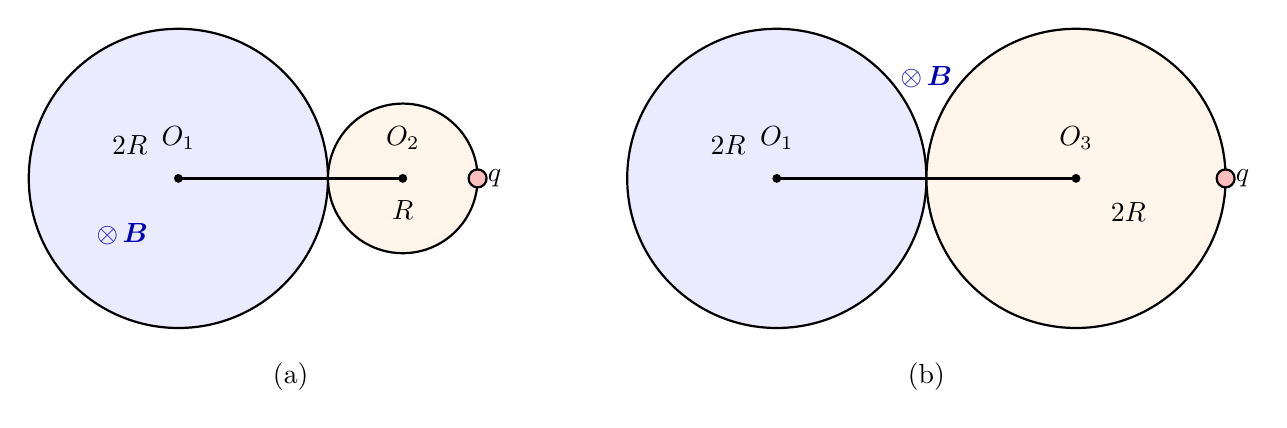
\begin{tikzpicture}[x=.95cm,y=.95cm]
  \begin{scope}[shift={(0,0)}]
    \draw[body] (0,0) circle(2);
    \draw[body,fill=orange!8] (3,0) circle(1);
    \draw[very thick] (0,0)--(3,0);
    \fill (0,0) circle(1.6pt) node[above=7pt]{$O_1$};
    \fill (3,0) circle(1.6pt) node[above=7pt]{$O_2$};
    \filldraw[fill=red!25,thick] (4,0) circle(.12) node[right]{$q$};
    \node at (-.65,.45){$2R$};
    \node at (3,-.42){$R$};
    \node at (1.5,-2.65){(a)};
    \node[blue!70!black] at (-.75,-.75){$\otimes\,\boldsymbol B$};
  \end{scope}
  \begin{scope}[shift={(8,0)}]
    \draw[body] (0,0) circle(2);
    \draw[body,fill=orange!8] (4,0) circle(2);
    \draw[very thick] (0,0)--(4,0);
    \fill (0,0) circle(1.6pt) node[above=7pt]{$O_1$};
    \fill (4,0) circle(1.6pt) node[above=7pt]{$O_3$};
    \filldraw[fill=red!25,thick] (6,0) circle(.12) node[right]{$q$};
    \node at (-.65,.45){$2R$};
    \node at (4.7,-.45){$2R$};
    \node at (2,-2.65){(b)};
    \node[blue!70!black] at (2.0,1.35){$\otimes\,\boldsymbol B$};
  \end{scope}
\end{tikzpicture}

% 04 question-07
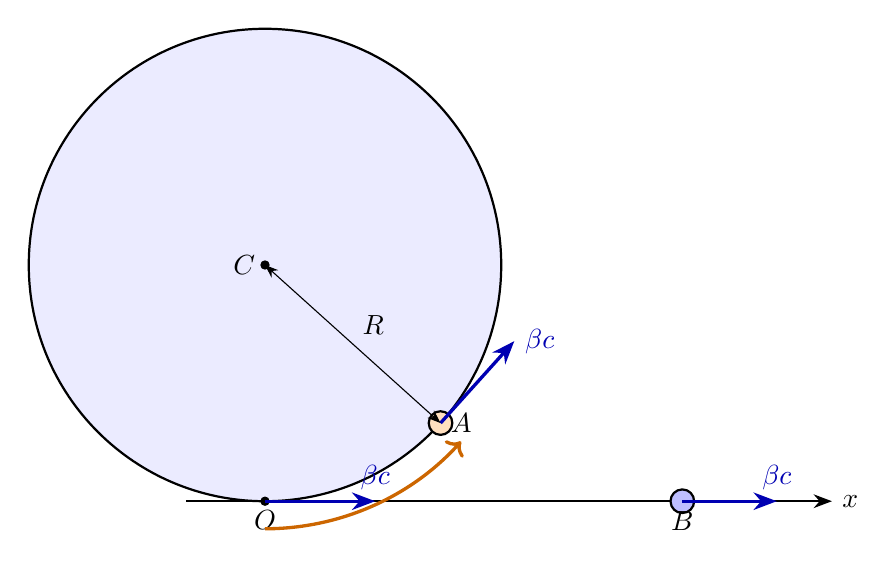
\begin{tikzpicture}[x=1cm,y=1cm]
  \coordinate (O) at (0,0);
  \coordinate (C) at (0,3);
  \draw[body] (C) circle(3);
  \draw[axis] (-1.0,0)--(7.2,0) node[right]{$x$};
  \fill (O) circle(1.7pt) node[below]{$O$};
  \fill (C) circle(1.7pt) node[left]{$C$};
  \coordinate (A) at ($(C)+(-42:3)$);
  \filldraw[fill=orange!25,thick] (A) circle(.15) node[right]{$A$};
  \filldraw[fill=blue!25,thick] (5.3,0) circle(.15) node[below]{$B$};
  \draw[velocity] (O)--++(1.4,0) node[above]{$\beta c$};
  \draw[velocity] (A)--++(48:1.4) node[right]{$\beta c$};
  \draw[velocity] (5.3,0)--++(1.2,0) node[above]{$\beta c$};
  \draw[dim] (C)--(A) node[midway,above right]{$R$};
  \draw[accent,->] ($(C)+(-90:3.35)$) arc[start angle=-90,end angle=-42,radius=3.35];
\end{tikzpicture}

% 05 solution-01
\begin{tikzpicture}[x=1cm,y=1cm]
  \begin{scope}[shift={(0,0)}]
    \coordinate (N0) at (0,0);
    \coordinate (Nx) at (4,0);
    \coordinate (V0) at (3.9,2.15);
    \coordinate (V1) at (.975,2.15);
    \draw[axis] (-.5,0)--(5.1,0) node[right]{法向 $n$};
    \draw[axis] (0,-.5)--(0,3.5) node[above]{切向 $t$};
    \draw[velocity] (0,0)--(3.9,2.15) node[above right]{$\boldsymbol v_0$};
    \draw[velocity,green!60!black] (0,0)--(.975,2.15) node[above]{$\boldsymbol v$};
    \draw[guide] (3.9,0)--(3.9,2.15);
    \draw[guide] (.975,0)--(.975,2.15);
    \draw pic[draw,"$\alpha$",angle radius=.85cm,angle eccentricity=1.25]
      {angle=Nx--N0--V0};
    \draw pic[draw,"$\alpha'$",angle radius=1.35cm,angle eccentricity=1.18]
      {angle=Nx--N0--V1};
    \node at (2.2,-1.0){等质量斜碰的速度分解};
  \end{scope}
  \begin{scope}[shift={(7.1,.3)}]
    \coordinate (Vx0) at (0,0);
    \coordinate (Vx1) at (5,0);
    \draw[axis] (-.7,0)--(6.2,0) node[right]{$v_x$};
    \draw[axis] (0,-2.1)--(0,2.7) node[above]{$v_y$};
    \coordinate (C) at (4.15,0);
    \draw[body,fill=orange!8] (C) circle(.83);
    \fill (C) circle(1.7pt) node[below]{$5v_0/6$};
    \draw[dim] (C)--++(0,.83) node[midway,right]{$v_0/6$};
    \coordinate (T) at ($(C)+(101.54:.83)$);
    \draw[velocity,purple!75!black] (0,0)--(T) node[above]{$\boldsymbol v$};
    \draw[guide] (C)--(T);
    \node at (1.65,.65){$\theta_{2\max}$};\draw pic[draw,angle radius=1.25cm]
      {angle=Vx1--Vx0--T};
    \node at (3.0,-2.55){完全弹性碰撞的速度圆};
  \end{scope}
\end{tikzpicture}

% 06 solution-02

\begin{tikzpicture}[x=.85cm,y=.85cm]
\begin{scope}
\draw[thick] (-2.5,0) arc(180:0:2.5);
\coordinate (C) at (0,0);\coordinate (O) at (55:3.1);\coordinate (T) at (0,3.1);
\draw[guide] (C)--(T);\draw[guide] (C)--(O);
\draw[body,fill=orange!10] (O) circle(.6);
\draw[force,red!70!black] (O)--++(55:1.2) node[right]{$N$};
\draw[force,blue!70!black] (O)--++(-90:1.4) node[below]{$mg$};
\draw[force,green!50!black] ($(O)+(235:.6)$)--++(145:1.1) node[left]{$f$};
\draw[velocity,purple!70!black] ($(O)+(0:1.2)$)--++(-35:1.1) node[right]{$\boldsymbol e_\theta$};
\draw pic[draw,"$\theta$",angle radius=.8cm]{angle=O--C--T};
\node at (.7,-1.1){(a) 固定基座；$\boldsymbol e_\theta$ 向右下};
\end{scope}
\begin{scope}[shift={(8.4,0)}]
\draw[very thick] (-2.7,0)--(3.8,0);\draw[thick] (-2.5,0) arc(180:0:2.5);
\coordinate (C) at (0,0);\coordinate (O) at (55:3.1);
\draw[guide] (C)--(O);\draw[body,fill=orange!10] (O) circle(.6);
\draw[velocity] (C)--++(-1.6,0) node[above]{$-v\hat{\boldsymbol x}$};
\draw[velocity,purple!70!black] (O)--++(-35:1.5) node[below right]{$L\dot\theta\boldsymbol e_\theta$};
\draw[force,gray!80!black] ($(O)+(0,.85)$)--++(1.4,0) node[above]{$ma\hat{\boldsymbol x}$};
\node[align=center] at (.7,-1.1){(b) 基座随动系；惯性力为 $ma\hat{\boldsymbol x}$\\$a=\dot v$ 为带符号量};
\end{scope}
\end{tikzpicture}

% 07 solution-03

\begin{tikzpicture}[x=.95cm,y=.95cm]
\begin{scope}
\draw[axis] (-3,0)--(3.4,0) node[right]{$x$};\draw[axis] (0,-2.8)--(0,3.1) node[above]{$y$};
\draw[thick] (0,0) circle(2.3);
\coordinate (O) at (0,0);\coordinate (X) at (3,0);\coordinate (Q) at (42:2.3);\coordinate (P) at (.7,-.4);
\fill (O) circle(1.5pt) node[below left]{$O$};\fill (Q) circle(2pt) node[above right]{$Q,\,\mathrm dq$};
\fill (P) circle(2pt) node[below]{$P_0(x,y,0)$};
\draw[velocity] (O)--(Q) node[pos=.65,above left]{$\boldsymbol r'$};
\draw[velocity,green!50!black] (O)--(P);
\draw[guide] (Q)--(P);
\draw pic[draw,"$\theta$",angle radius=.8cm]{angle=X--O--Q};
\node[align=center] at (.2,-3.7){(a) $xOy$ 面内投影\\$A=\hat{\boldsymbol r}'\cdot\boldsymbol\rho=x\cos\theta+y\sin\theta$};
\end{scope}
\begin{scope}[shift={(8.5,0)}]
\draw[thick] (-2.3,0) ellipse(2.3 and .7);
\coordinate (O) at (-2.3,0);\coordinate (P0) at (-1.3,-.2);\coordinate (P) at (-1.3,1.5);
\draw[axis] (O)--++(0,2.8) node[above]{$z$};
\draw[guide] (P0)--(P);\fill (P0) circle(2pt) node[below]{$P_0$};\fill (P) circle(2pt) node[right]{$P(x,y,z)$};
\draw[velocity,green!50!black] (O)--(P) node[midway,left]{$\boldsymbol\rho$};
\draw[dim] (-.4,-.2)--(-.4,1.5) node[midway,right]{$z$};
\node[align=center] at (-2.2,-3.7){(b) 离面场点的投影\\$\rho^2=x^2+y^2+z^2$；$\boldsymbol r'\cdot\boldsymbol\rho=rA$};
\end{scope}
\end{tikzpicture}

% 08 solution-04

\begin{tikzpicture}[x=.85cm,y=.85cm]
\begin{scope}
\draw[body] (0,0) circle(2);\draw[axis] (-2.7,0)--(2.7,0) node[right]{$x$};
\draw[accent] (.8,0) ellipse(.4 and 1.833);
\draw[dim] (0,0)--(.8,1.833) node[midway,left]{$R$};
\draw[force,purple!70!black] (0,-2.6)--(-2,-2.6) node[midway,below]{$\boldsymbol m_0\parallel\boldsymbol\omega$};
\node at (-.8,1){$+Q_0$};\node at (.8,2.4){纬带电流环};
\node at (0,-3.5){(a) 正电荷的磁矩沿 $-x$};
\end{scope}
\begin{scope}[shift={(6.4,0)}]
\draw[axis] (-.4,0)--(5.6,0) node[right]{$x$};\draw[axis] (0,-.4)--(0,4.5) node[above]{$y$};
\coordinate (O) at (0,0);\coordinate (X) at (5,0);\coordinate (P) at (3,3);
\draw[guide] (O)--(P);\draw[guide] (3,0)--(P);\fill (P) circle(2pt) node[above right]{$-q$};
\node[blue!70!black] at (3.6,2.7){$\otimes\,\boldsymbol v$};
\draw[force,red!70!black] (P)--++(-1.3,-1.3) node[left]{$\boldsymbol F_E$};
\draw[force,green!50!black] (P)--++(1.3,-.43) node[right]{$\boldsymbol F_B$};
\draw[force] (P)--++(0,-2.2) node[right]{$\boldsymbol F_{\rm net}$};
\draw pic[draw,"$\theta$",angle radius=.8cm]{angle=X--O--P};
\node[align=center] at (2.5,-3.5){(b) 子午面分解示意，$\theta=45^\circ$\\$F_x=0$；$F_y=-m\omega'^2r\sin\theta$};
\end{scope}
\end{tikzpicture}

% 09 solution-05

\begin{tikzpicture}[x=.9cm,y=.9cm]
\begin{scope}
\coordinate (O) at (0,0);\coordinate (X) at (4,0);\coordinate (C) at (35:3);\coordinate (Q) at ($(C)+(105:1)$);
\draw[body] (O) circle(2);\draw[body,fill=orange!8] (C) circle(1);\draw[thick] (O)--(C);
\draw[guide] (O)--(Q);\fill (Q) circle(2pt) node[above]{$q$};
\draw[dim] (O)--(C) node[pos=.5,above left]{$3R$};\draw[dim] (C)--(Q) node[midway,left]{$R$};
\draw pic[draw,"$\theta$",angle radius=.65cm,angle eccentricity=1.35]{angle=X--O--C};
\draw pic[draw=orange!80!black,"$\theta'$",angle radius=1.45cm,angle eccentricity=1.2]{angle=X--O--Q};
\coordinate (CX) at ($(C)+(1.4,0)$);\draw[guide] (C)--(CX);
\draw pic[draw=purple!70!black,"$\varphi$",angle radius=.42cm,angle eccentricity=1.6]{angle=CX--C--Q};
\draw[velocity] (Q)--++(-1,.8) node[left]{$\boldsymbol E_\varphi$};
\node[align=center] at (1,-3){(a) 固定大环：$\varphi=3\theta$\\$\boldsymbol r_q=3R\boldsymbol e(\theta)+R\boldsymbol e(\varphi)$};
\end{scope}
\begin{scope}[shift={(7.5,-1.2)}]
\draw[axis] (0,0)--(6.3,0) node[right]{$\rho/a_B$};\draw[axis] (0,0)--(0,4) node[above]{$E_\varphi/(ka_B/2)$};
\draw[thick,blue!70!black] (0,0)--(2,3);
\draw[thick,blue!70!black,domain=2:5.7,samples=70] plot(\x,{6/\x});
\draw[guide] (2,0)--(2,3);\node[below] at (2,0){$1$};\node[left] at (0,3){$1$};
\node[above,align=center] at (3.4,3.8){磁通区半径为 $a_B$};
\node[align=center] at (3.4,-1.8){(b) $\rho\le a_B$: $E_\varphi=k\rho/2$\\$\rho\ge a_B$: $E_\varphi=ka_B^2/(2\rho)$};
\end{scope}
\end{tikzpicture}

% 10 solution-06

\begin{tikzpicture}[x=1cm,y=1cm]
\draw[axis] (0,0)--(9.3,0) node[right]{$V$};\draw[axis] (0,0)--(0,5) node[above]{$p_w$};
\draw[very thick,red!70!black] (2.15,4)--(4.3,4);
\draw[thick,blue!70!black,domain=4.3:8.6,samples=80] plot(\x,{17.2/\x});
\foreach \x/\y/\label in {2.15/4/{V_1/4},4.3/4/{V_s=V_1/2},8.6/2/{V_1}}{
\draw[guide] (\x,0)--(\x,\y);\fill (\x,\y) circle(2pt);\node[below] at (\x,0){$\label$};}
\draw[guide] (0,4)--(4.3,4);\draw[guide] (0,2)--(8.6,2);
\node[left] at (0,4){$p_s=p_1$};\node[left] at (0,2){$p_1/2$};
\node[red!70!black] at (2.9,4.65){凝结段};\node[blue!70!black] at (6.6,3.7){未饱和：$p_wV=n_wRT_1$};
\draw[force,orange!80!black] (8,.9)--(2.5,.9) node[midway,above]{压缩方向};
\end{tikzpicture}

% 11 solution-07

\begin{tikzpicture}[x=1.3cm,y=1.3cm]
\def\be{0.6}\def\ta{1.5}\pgfmathsetmacro\psiDeg{\be*\ta*180/pi}
\pgfmathsetmacro\xa{sin(\psiDeg)}\pgfmathsetmacro\ba{\ta-\be*\xa}
\pgfmathsetmacro\tb{\ba/(1-\be*\be)}
\begin{scope}
\draw[axis] (0,0)--(2.3,0) node[right]{$x/R$};\draw[axis] (0,0)--(0,3.3) node[above]{$ct/R$};
\draw[thick,blue!70!black] (0,0)--({\be*3.05},3.05) node[above right]{$B$};
\draw[thick,orange!80!black,domain=0:3.05,samples=90] plot({sin(\be*\x*180/pi)},\x);
\node[orange!80!black,right] at (1,2.7){$A$ 的 $x$ 投影};
\coordinate (PA) at (\xa,\ta);\coordinate (PB) at ({\be*\tb},\tb);
\draw[purple!70!black,thick] (0,\ba)--(2.1,{\ba+\be*2.1});
\fill (PA) circle(1.8pt) node[above left]{$P_A$};\fill (PB) circle(1.8pt) node[below right]{$P_B$};
\node[align=center] at (1.1,-.85){(a) $B$ 系同时线\\$ct-\beta x=$ 常量};
\end{scope}
\begin{scope}[shift={(4.0,0)}]
\pgfmathsetmacro\cp{cos(\psiDeg)}\pgfmathsetmacro\sp{sin(\psiDeg)}
\pgfmathsetmacro\xiPlot{\cp*sin(\psiDeg)+\sp*(1-cos(\psiDeg))}
\pgfmathsetmacro\inter{\ta-\be*\xiPlot}
\pgfmathsetmacro\TB{\inter/(1-\be*\be*\cp)}
\draw[axis] (0,0)--(2.3,0) node[right]{$\xi/R$};\draw[axis] (0,0)--(0,3.3) node[above]{$ct/R$};
\draw[thick,blue!70!black] (0,0)--({\be*\cp*3.05},3.05) node[above right]{$B$};
\draw[thick,orange!80!black,domain=0:3.05,samples=90] plot({\cp*sin(\be*\x*180/pi)+\sp*(1-cos(\be*\x*180/pi))},\x);
\coordinate (PA) at (\xiPlot,\ta);\coordinate (PB) at ({\be*\cp*\TB},\TB);
\draw[purple!70!black,thick] (0,\inter)--(2.1,{\inter+\be*2.1});
\fill (PA) circle(1.8pt) node[above left]{$P_A$};\fill (PB) circle(1.8pt) node[below right]{$P_B$};
\node[align=center] at (1.1,-.85){(b) $A$ 瞬时同时线\\$ct-\beta\xi=$ 常量};
\end{scope}
\node[align=center] at (3.0,-1.8){示例 $\beta=0.6$，$ct_A/R=1.5$；$\xi=\boldsymbol n_A\cdot\boldsymbol r$\\$\boldsymbol n_A=(\cos\psi,\sin\psi)$，各事件点由方程求交得到};
\end{tikzpicture}

% 12 solution-08

\begin{tikzpicture}[x=.8cm,y=.8cm]
\begin{scope}
\draw[axis] (-3,0)--(3.3,0) node[right]{$p_x'$};\draw[axis] (0,-2.9)--(0,3.1) node[above]{$p_y'$};
\draw[thick] (0,0) circle(2.3);
\draw[velocity,purple!70!black] (0,0)--(160:2.3) node[above left]{$\boldsymbol p_R'$};
\draw[velocity,green!50!black] (0,0)--(-20:2.3) node[below right]{$\boldsymbol p_{ee}'$};
\node[align=center] at (0,-3.7){(a) 总质心系\\$\boldsymbol p_R'+\boldsymbol p_{ee}'=0$};
\end{scope}
\begin{scope}[shift={(7.6,0)}]
\def\d{3.05}\def\a{2.7}\def\b{2.5}
\pgfmathsetmacro\tx{\d-\a*\a/\d}\pgfmathsetmacro\ty{\b*sqrt(1-\a*\a/(\d*\d))}
\draw[axis] (-.5,0)--(6.3,0) node[right]{$p_x$};\draw[axis] (0,-2.9)--(0,3.1) node[above]{$p_y$};
\draw[thick,blue!70!black] (\d,0) ellipse[x radius=\a,y radius=\b];
\coordinate (O) at (0,0);\coordinate (X) at (5,0);\coordinate (T) at (\tx,\ty);
\draw[velocity,purple!70!black] (O)--(T) node[above left]{$T$};\fill (T) circle(2pt);
\draw[guide] (\d,0)--(T);\fill (\d,0) circle(1.5pt) node[below]{$d$};
\draw pic[draw,"$\theta_M$",angle radius=.7cm,angle eccentricity=1.3]{angle=X--O--T};
\node[align=center] at (2.6,-3.7){(b) 椭圆切线示意，尺度未按本题数值\\$d=\gamma_C\beta_CE_n'$，$a=\gamma_Cp_R'$，$b=p_R'$};
\end{scope}
\end{tikzpicture}

\end{document}
